\documentclass[eso]{bcc}
\usepackage{setspace}
\usepackage[indentfirst=false,rightmargin=0cm,leftmargin=4cm]{quoting}
\titulo{Implantação do gerenciamento de configuração e da central de serviços alinhados as melhores práticas da ITIL}
\palavrasChave{ITIL}{Gerenciamento}{Implantação.}
\keywords{ITIL, Management, Implantation.}

\autor{Eduardo Ferreira Felix}{eduardofelix1221@gmail.com}

\orientador{Dr. Asssuero Fonseca Ximenes}{UAG}{UFRPE}
%\orientadorDois{John von Neumann}{UAG}{UFRPE}
% \orientadorTres*{Ada Lovelace}{UAG}{UFRPE} % Se feminino use *, tanto para orientador ou examinador

\examinador*{Msc. Kádna Maria Alves Camboim Vale}{UAG}{UFRPE}
\examinadorDois{Thiago Monteiro de Melo}{Colégio Damas Santa Sofia}{ARIC}
%\examinadorTres{Stephen Cook}{UAG}{UFRPE}
%\examinadorQuatro{John Backus}{UAG}{UFRPE}

\dataMesAno{25}{Janeiro}{2018}


\empresaNome{Asssociação das Religiosas da Instrução Cristã}
\empresaArea{Educação}
\empresaPeriodo{1 de novembro a 25 de janeiro de 2018}
\empresaCargaH{30H}
\empresaRemuneracao{Não remunerado}
\empresaSupervisorEmail{Thiago Monteiro de Melo/thiago.monteiro@colegiosantasofia.com.br }
\logo{Figuras/logocolegio}{1}

\begin{document}

\selectlanguage{portuguese}

\capa

% \capaDois

\begin{resumo}
Nesse relatório é apresentado como foi efetuado o processo de implantação do gerenciamento de configuração e o processo da central de serviços que seguiu as práticas propostas pela ITIL, no Colégio Damas Santa Sofia, que se situa na cidade de Garanhuns- PE. Essa implantação se justificou por possibilitar a organização um controle de todos os seus ativos de tecnologias, além de ter uma central de serviços que oferece, aos usuários, mais praticidade e facilidade na abertura de chamados para a solução dos problemas/incidentes que possam acontecer na sua estrutura. 
Por meio do gerenciamento de configuração, o setor de TI da empresa terá um controle de onde estão localizados todos seus ativos  permitindo a localização  de cada item de configuração. Com a utilização da central de serviços, a empresa proporcionará aos seus colaboradores uma forma de acompanhar os chamados por meio da rede de internet, como também gerar relatórios de atendimentos e resolução de incidentes de forma mais rápida. 
Dentre os benefícios com essa implantação destaca-se a praticidade, a agilidade no atendimento e o controle dos itens de configuração. Para a operacionalização dessa implantação foi utilizado o software ITOP, em conjunto com o servidor wampserver, que possui integração com o PHP, mySQL e o apache e, além disso, segue algumas diretrizes da biblioteca ITIL. 
\end{resumo}


\selectlanguage{english}
\begin{abstract}

This report presents how the implementation of the configuration management process and the service center process that followed the practices proposed by ITIL, at the Damas Santa Sofia College, located in the city of Garanhuns-PE, was performed. This implementation was justified by allowing the organization to control all of its technology assets, as well as having a service center that offers users more practicality and ease in opening calls for the solution of problems / incidents that may occur in the structure.
By means of configuration management, the company's IT sector will have a control of where all its assets are located, allowing the location of each configuration item. With the use of the service center, the company will provide its employees with a way to follow the calls through the internet network, as well as generate reports of attendance and resolution of incidents more quickly.
Among the benefits with this deployment is the practicality, the agility in attendance and the control of the configuration items. For the implementation of this deployment, ITOP software was used in conjunction with the wampserver server, which has integration with PHP, mySQL and apache, and also follows some ITIL library guidelines.
\end{abstract}

\selectlanguage{portuguese}

% Centralizar titulos
\renewcommand\contentsname{\centerline{Sumário}}
\renewcommand\listfigurename{\centerline{Lista de Figuras}}
\renewcommand\listtablename{\centerline{Lista de Tabelas}}

\lhead{Sumário}
\tableofcontents

\listoffigures
\addcontentsline{toc}{chapter}{Lista de Figuras}

\listoftables
\addcontentsline{toc}{chapter}{Lista de Tabelas}

\inicio
\chapter{Introdução}

O Estágio Supervisionado Obrigatório (ESO)  proporciona a oportunidade de exercitar,  na prática, os conhecimentos adquiridos em sala de aula ao longo dos anos de graduação. O estagiário ao compartilhar os processos executados em uma empresa tem a possibilidade de ter contato com diversos profissionais que atuam em diversas áreas do conhecimento e, por isso, esse contato é de suma importância para inserção do estagiário no mercado de trabalho adquirindo experiência nas rotinas das organizações. 

Além disso, o estudante possibilita a empresa conhecimentos recentes  discutidos na universidade e, dessa foma, ocorre uma troca de saberes. Diante disso,foi possível verificar que, com a implantação das diretrizes da biblioteca ITIL, a empresa ganhou tempo na execução das demandas internas e externas, adquiriu mais agilidade na tomada de decisão e solução de problemas, aumentou os níveis de satisfação dos usuários, conseguiu redução dos custos operacionais e melhorou o nível de otimização da organização.


 O Colégio Santa Sofia possui diversos setores e tem o setor de TI como responsável por dar suportes tecnológicos  a todos eles.  De acordo com as observações da rotina  diária dos funcionários do setor de TI, percebeu-se a necessidade da implantação do gerenciamento de itens de configuração, pois não era realizado nenhum controle sobre os ativos. Além disso verificou-se a necessidade de implantação de uma central de serviços, uma vez que não existia processos para o agendamento de chamados e geração de relatório de atendimento.

Ao longo do ESO, foi possível aprimorar os conhecimentos adquiridos  a respeito da biblioteca ITIL, além de proporcionar a oportunidade de aprender na prática como ocorre o processo de implantação do gerenciamento de configuração e da central de serviços.É importante salientar que o ITIL é um guia para gerenciar todos os serviços de TI e que o mesmo não se limita a estas duas gerências. Mas pelo fato da organização não possuir nenhum controle, como passo inicial foi adotado a implantação dessas duas gerências para que, no futuro, as outras gerências possam ser implementadas.


\section {Objetivo geral}

Efetuar a implantação do gerenciamento de configuração e da central de serviços seguindo a metodologia da biblioteca ITIL.

\subsection{Objetivos específicos}

\begin{itemize}

\item Apresentar conceitos e boas práticas de gerenciamento de serviços de TI;
\item Etiquetar e organizar todos os itens de configuração da empresa;
\item Inserir todos os ativos de TI no banco de dados de gerenciamento de itens de configuração;
\item Implantar o gerenciamento de configuração e a central de serviços  usando o software Itop seguindo as boas práticas da ITIL;
\item Treinar e elaborar um manual de uso dos sistemas de apoio da central de serviços e do gerenciamento de configuração para ser utilizado pelos técnicos no atendimento de chamados e na inserção de dados no banco de dados de gerenciamento de itens de configuração;

\end{itemize}

\section{Justificativa}

Uma das principais vantagens da ITIL é a sua flexibilidade. Não há  necessidade da organização adotar todos os métodos e rotinas definidas pela política de gestão para que ela possa ter melhorias nos seus processos internos, embora que caso sejam adotadas, a organização terá muito mais controle nos seus processos. Assim, a ITIL pode ser aplicada em diferentes realidades e mercados com facilidade. Com a implantação da ITIL na organização houve uma redução de custos operacionais que impactou na melhoria da competitividade do negócio, além de proporcionar uma  eficiência interna que foi ampliada por meio da racionalização de processos de TI e pelo alinhamento dos recursos digitais por meios das melhores estratégias de mercado em relação a gestão de serviços de TI.

A partir dos estudos das necessidades da empresa em relação ao setor de TI, percebeu-se que não existia nenhum controle dos seus ativos tecnológicos, como também sobre os chamados feitos pelos colaboradores. Diante de tais necessidades, surgiu a ideia de implantar o gerenciamento de configuração e a central de serviços seguindo as boas práticas adotadas pela ITIL. 

Com uma Central de Serviços a empresa pode proporcionar aos seus usuários um nível de serviço de qualidade e atendimento dentro dos padrões internacionais de prestação de serviços. Uma possível definição para o serviço ao cliente ou usuário é definida por Uttal e Davidow (1991) como: “Serviço ao cliente significa todos os aspectos, atitudes e informações que ampliem a capacidade do cliente de compreender o valor potencial de um bem ou serviço essencial.” Apud \cite[p.45]{magalhaes:2007}.  Assim, a central de serviço proporciona benefícios para a empresa de forma significativa, elevando o índice de satisfação dos usuários e a resolução dos incidentes de forma mais rápida, tornando-se um ponto único de contatos entre os usuários da instituição.

Para Magalhães e Pinheiros, “muitas áreas de TI estão iniciando um movimento para se tornarem orientadas a serviços sem uma clara visão do escopo, dos riscos e do retorno desta nova abordagem. Como resultado, a taxa de falhas é expressiva e, a cada dia que passa, mais visível.”\cite[p.37]{magalhaes:2007}. Assim sendo, é de suma importância o acompanhamento dos serviços na empresa com o objetivo de orientar e treinar os funcionários responsáveis pela execução, contribuindo para um gerenciamento de serviços de qualidade, que proporcione satisfação e segurança aos seus usuários. É válido salientar, a importância da satisfação dos usuários em utilizar os serviços oferecidos e a satisfação dos técnicos em trabalhar com a central de serviços. A metodologia ITIL possibilita garantir a satisfação de ambas as partes, além de colocar a empresa em um patamar  elevado em relação aos serviços de TI.

Em uma empresa é  fundamental  o acompanhamento dos ativos de TI, por isso se faz necessário saber a  localização de  onde estão todos os seus itens de configuração, principalmente, se a empresa for de grande porte. Seguindo as boas práticas da biblioteca ITIL, é possível que se tenha um acompanhamento de todos os itens de configuração de uma organização. Dessa forma, se faz necessário a criação de uma base de dados, na qual será inseridos todos os ativos tecnológicos da instituição, de forma que possa ter um melhor controle de suas localizações geográficas. Para dar início a criação de uma   base de dados do processo de gerenciamento da configuração é preciso que todos os itens da corporação estejam etiquetados, para facilitar a sua inserção no banco de dados. Segundo \cite[p.91]{filho:2011}, “O sistema de gerenciamento de configuração (SGC) mantém os relacionamentos entre todos os componentes do serviço e qualquer documentação de incidentes, problemas, erros conhecidos, mudanças e liberações”. Assim sendo, a implantação de um gerenciamento de configuração  dará subsídios para implementação de novas gerências. 

Para possibilitar a utilização com conceitos do ITIL foi utilizado o software ITOP  por se tratar de um software que atende a demanda da empresa e ser de fácil manuseio. Em relação aos benefícios proporcionados para empresa esse projeto ampliou a visão de como gerenciar os seus serviços de TI, garantir a eficiência em seus processos, satisfação dos seus clientes e a redução de custos. Já para o discente possibilitou  a oportunidade de colocar em prática os conhecimentos adquiridos durante a graduação. 

\section{A empresa}
O Colégio Damas Santa Sofia  é uma instituição de ensino da ARIC–Associação das Religiosas da Instrução Cristã fundada em 1823, na Bélgica, por Madre Agathe Verhelle. Após várias fundações na Europa, o Instituto expandiu-se pela América do Sul e África e chegou ao Brasil em 1896, na cidade de Olinda, no estado de Pernambuco, instalando-se, posteriormente, no Recife e em outras cidades em diversos estados brasileiros . 

O Colégio Damas Santa Sofia, localiza-se na rua Nilo Peçanha,20, Santo Antônio na cidade de Garanhuns, fundado no ano de 1912 pelo Monsenhor Afonso Pequeno, vigário da matriz de Santo Antônio. Associação das Religiosas da Instrução Cristã - ARIC é a mantenedora das instituições educacionais da Rede Damas de Ensino. Orientada pelas Religiosas da Instrução Cristã. A ARIC segue os legados e ensinamentos deixados pela Me. Agathe Verhelle, fundadora da Congregação Damas.
A imagem \ref{UCrede} representa como a rede damas está distribuida no mundo.

\newpage

\begin{figure}[!h]
\centering
\caption[Rede Damas]{Rede Damas.}
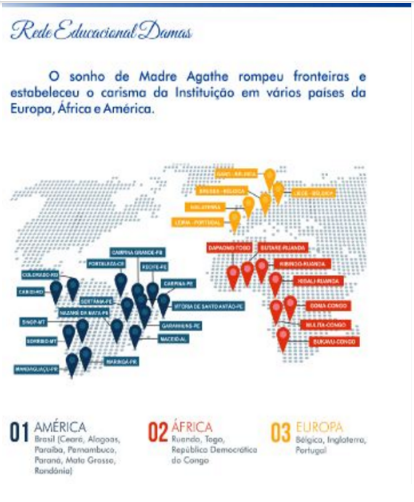
\includegraphics[scale=1.3]{Figuras/rededamas.png}
\label{UCrede}
\end{figure}

\subsection{Colégio Damas Santa Sofia}

O colégio Santa Sofia, fundado na cidade de Garanhuns  em 18 de setembro de 1912, tem uma equipe de 141 funcionários e 1300 estudantes, oferecendo ensino infantil, ensino fundamental I, ensino fundamental II e ensino médio. 
Na imagens \ref{UCfachada} é possível ver a fachada do colégio.

\newpage

\begin{figure}[!h]
\centering
\caption[Fachada Colégio]{Fachada do Colégio Damas Santa Sofia.}
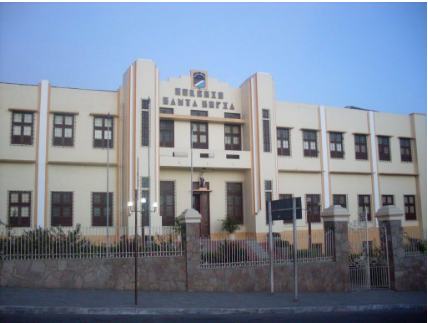
\includegraphics[scale=1.3]{Figuras/fachadacolegio.png}
\label{UCfachada}
\end{figure}
\subsection{Fundação da Rede Damas}
O  Instituto das Religiosas da Instrução foi fundado por Inês Margarida Verhelle (Madre Agathe) no ano de 1823 na Bélgica.  Madre Agathe batalhou  por seis anos no ideal de tornar-se religiosa, enfrentando inclusive a oposição aberta de sua família, porém o chamado de Deus foi mais forte. Em 18 de julho de 1815, aos 29 anos deixou secretamente a família e ingressou na vida religiosa, mas suas dificuldades continuaram, destacando-se o fechamento da instituição na qual ingressou. No entanto,oito meses após o fechamento pelo rei Guilherme I da Holanda, Madre Agathe funda uma nova Instituição, que coloca o nome de  Instituto das Damas da Instrução Cristã.
Madre agathe tinha o sonho de revelar a face do Cristo educador à juventude, disposta a continuar o seu trabalho, funda na Europa, os colégios de Vracene (1827), Audenarde (1828), Bruges (1829), Renaix (1832), Anvers (1834), Gand (1838) e Liege (1838) . Após a sua morte, em 1858, o Instituto consolidado expande-se pelos continentes Sul-Americano e Africano. A imagem \ref{UCmadre} mostra a fundadora da rede damas.

\newpage

\begin{figure}[!h]
\centering
\caption[Madre Agathe]{Madre Agathe Verhelle.}

\includegraphics[scale=1.3]{Figuras/madre.png}
\label{UCmadre}
\end{figure}
\subsection{Damas no Brasil}
Dando continuidade aos ideais de Madre Agathe, o grupo formado por nove mulheres enfrentou três meses de viagem para instalar-se no Brasil. Em 15 de outubro de 1896, orientadas por Madre Loyola, as primeiras representantes da Congregação Damas chegaram ao porto do Recife, estabeleceram-se em Olinda no Convento de São Francisco - primeira casa da Congregação no Brasil - que oferecia aulas de música ao internato. Durante as primeiras oito décadas de funcionamento no Brasil, o Instituto das Damas dedicou-se exclusivamente a educação feminina, aspecto que viria a modificar-se com a adoção do ensino para ambos os sexos em 1970. Após a fundação do Colégio Damas no Recife, outros colégios nasceram como é o caso do colégio Santa Sofia na cidade de Garanhuns.

\section{Organização do relatório}

A organização desse relatório segue a seguinte forma: o \autoref{chap:fundamentacao} apresenta a fundamentação teórica dos conceitos utilizados nas atividades desenvolvidas; o \autoref{chap:atividades} apresenta o detalhamento das atividades desenvolvidas  e, por fim, o \autoref{chap:conclusao} mostra a conclusão do trabalho realizado e os resultados obtidos.

\chapter{Fundamentação Teórica}
\label{chap:fundamentacao}

Nesta seção são apresentados conceitos utilizados no desenvolvimento deste projeto e suas respectivas justificativas para o uso dos mesmos.

\section{A ITIL}
ITIL é a sigla para \textit{ Information Technology Infrastructure Library}, que em uma tradução livre para a língua portuguesa, significa biblioteca de infraestrutura de Tecnologia da Informação, ou seja, um conjunto das melhores práticas para a gestão de serviços em TI e o alinhamento dessa área com os negócios da empresa.

A ITIL apresenta a definição dos processos de estratégia, desenho, transição, operação e melhoria contínua dos serviços necessários para o gerenciamento de TI aplicados a empresa. Para \cite[p.65]{magalhaes:2007}, “ a ITIL não define os processos a serem implantados na área de TI, mas, sim, demonstrar as melhores práticas que podem ser utilizadas para esta definição”.  É válido salientar que, a adoção das práticas da ITIL pode ser incorporada na empresa conforme for surgindo a necessidade de inclusão.

\subsection{Gerenciamento de processos}

A ITIL faz o gerenciamento de TI baseando-se em processos. Para a ITIL, trabalhar com processos é de suma importância para agregar valor para a organização. \cite[p.65]{magalhaes:2007}, afirma que: “ um processo pode tornar-se bastante complexo, dependendo da organização, sendo que, para cada processo, existe um método de gerenciamento específico”. Assim, é relevante estudar como acontece o funcionamento dos processos e como ocorre a interligação entre eles. 

Segundo\cite[p.65]{magalhaes:2007}, os objetivos do gerenciamento de processos são: “aumentar a qualidade dos serviços; aumentar a previsibilidade do comportamento; diminuir o custo alocado. ” Dessa forma, fica evidente que uma empresa que gerencia os seus processos só tem a ganhar, uma vez que colocar a empresa em um patamar mais elevado.

\subsection{Modelo de referência e a ITIL}

A ITIL considera relevante dentro da organização um planejamento para tais itens:  gerenciamento de configuração, central de serviços, gerenciamento de incidentes, gerenciamento de problemas, gerenciamento de mudanças, gerenciamento de liberação, gerenciamento do nível de serviço, gerenciamento de capacidade, gerenciamento da disponibilidade, gerenciamento da continuidade dos serviços de TI e gerenciamento financeiro. Em suma, ela apresenta um passo-a-passo de como estes gerenciamentos devem serem implementados.

A metodologia ITIL diferencia por duas grandes áreas de atuação nos processos de gerenciamento de serviços: entrega dos serviços e suporte ao serviço. Para \cite[p. 67]{magalhaes:2007}:

\begin{quoting}
{\footnotesize
Os processos da área de suporte ao serviço concentram-se nas tarefas de execução diárias, necessárias para manutenção dos serviços de TI já entregues e em utilização pela organização. São eles:Gerenciamento de Configuração (Configuration Management);Gerenciamento de Incidente ( Incident Management); Gerenciamento de Problema ( Problem Management);Gerenciamento de Mudança (Change Management); Gerenciamento de Liberação (Release Management);}
\end{quoting}
Diante disso, compreender como funciona cada processo é de extrema importância para o êxito da inserção da ITIL na organização, tornando-se bastante relevante para saber como ocorre o mecanismo de troca de informação entre os processos e como eles estão conectados entre si. Dessa forma, é possível identificar o que cada gerência faz, como usufruir de cada uma delas da melhor forma possível. A partir da ciência sobre a área de suporte ao serviço  e dos processos que a compoem, o gestor de TI terar mais preparo para lidar com imprevisto que venha ocorrer no dia-a-dia.
É válido ressaltar, os processos da área de entrega ao serviço e quais gerenciais fazem parte dela. Para \cite[p. 67]{magalhaes:2007}: 
\begin{quoting}
{\footnotesize
Os processos desta área concentram-se nas atividades de planejamento a longo prazo dos serviços que serão demandados pela organização e na melhoria dos serviços já entregues e em utilização pela organização. São eles: Gerenciamento do Nível de Serviço (Service Level Management); Gerenciamento de Capacidade (Capacity Management); Gerenciamento da Disponibilidade ( Availability Management); Gerenciamento da Continuidade dos Serviços de TI (IT Service Continuity Management); Gerenciamento Financeiro (Financial Management);
}
\end{quoting}

Assim, tendo conhecimento de como empregar todos esses conceitos o gestor de TI poderá padronizar os procedimentos para o pessoal de TI e definir as melhores práticas, uma vez que a metodologia ITIL proporciona uma significativa melhora na qualidade da comunicação, compartilhamento e disponibilização das informações.

Dentre as vantagens da implantação da ITIL estão: a redução no tempo de execução das demandas internas e externas; mais agilidade na tomada de decisão e solução de problemas; e, em especial, o aumento dos níveis de satisfação dos clientes e usuários. Tudo isso, através de uma estratégia de redução dos custos operacionais e de otimização da organização e gestão dos processos do setor de tecnologia da informação.
Na figura \ref{UCmodelo} abaixo tem-se a visão geral do modelo de referência de processos de TI segundo a biblioteca ITIL.

\newpage

\begin{figure}[!h]
\centering
\caption[Modelo de referência]{Modelo de referência de processos de TI segundo a biblioteca ITIL.}
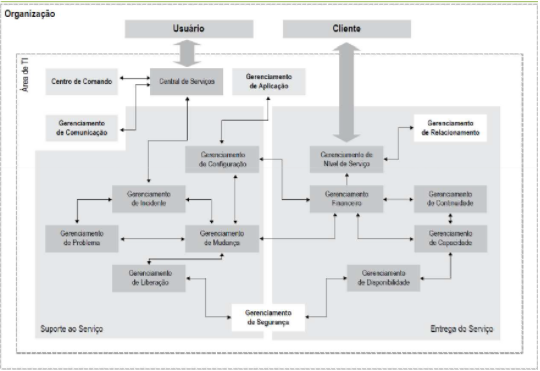
\includegraphics[scale=1]{Figuras/modelo.png}
\label{UCmodelo}
\end{figure}

\subsection{Gerenciamento de configuração}

O Gerenciamento de Configuração fornece informações seguras e atualizadas sobre os Itens de Configuração (IC's) em uso, assegurando o inter-relacionamento direto com as demais disciplinas de gerenciamento de serviços da TI na organização. Dessa forma, é possível dar um suporte aos processos de Gerenciamento de Serviços fornecendo informações precisas da configuração, permitindo, assim, uma tomada de decisão mais assertiva e em tempo hábil – por exemplo, para autorização de mudanças e liberações ou resolver incidentes e problemas.

Nessa perspectiva, a criação de um banco de dados de itens de configuração constará as especificações e localizações dos itens, proporcionando uma melhor integração de forma que venham contribuir de maneira significativa para a empresa. A implantação do gerenciamento de configurações permite identificar e tratar erros na infraestrutura da empresa, entre outros problemas e incidentes que possam vir a ocorrer. 

\cite[p.90]{filho:2011} afirma que os principais objetivos do processo de gerenciamento de configuração são: “fornecer gerenciamento da TI com maior controle sobre os ICs da organização; fornecer informações precisas a outros processos da ITIL; criar e manter uma base de dados do gerenciamento da configuração (BDGC) ”. Dessa forma, a implantação do gerenciamento de configuração proporcionará para a empresa um maior controle dos seus ativos de TI. Esse acompanhamento será um dos fatores primordiais para redução de gastos, proporcionando para o gestor de TI o entendimento sobre como investir e quando investir em ativos.

Contudo, entender o que são itens de configuração e como organizá-los é de suma importância para que ocorra de maneira efetiva e com sucesso a implementação da ITIL. Segundo \cite[p. 69]{magalhaes:2007}: “ Um item de configuração é um componente que faz parte ou está diretamente relacionado com a intra-estrutura de TI. Um item de configuração pode ser um componente físico ou lógico, bem como pode também ser composto por outros itens de configuração”. Identificando os ativos de TI, criando categorias, organizando os itens de configuração que são compostos por outros itens ajuda a gerenciá-los melhor, tornando até mais fácil de localizá-los. Assim,com a implantação do gerenciamento de configuração o setor de TI  se beneficia em amplos sentidos, além de agregar valor aos usuários dos ativos de TI da organização. 

Através da catalogação e documentação de todos os equipamentos, ativos e demais itens de configuração existentes na empresa, é possível obter um controle maior sobre todos os itens. Como esta é a gerência principal para a implementação do restante do ITIL, a empresa necessita primordialmente adotá-la para seguir com a implementação das outras gerências. Para \cite[p. 88]{magalhaes:2007}:
\begin{quoting}
{\footnotesize
 O estabelecimento de uma BDGC e do processo de gerenciamento de configuração traz uma série de benefícios à área de TI e, por consequência, a organização, destacando-se: fornecimento de informações precisas sobre os itens de configuração e respectiva documentação para apoiar todos os demais processos descritos na ITIL. Especificação da versão, da propriedade e da informação relativa ao estado para os itens de configuração.
}
\end{quoting}

A partir da criação do banco de dados do gerenciamento de configuração (BDGC) e do processo de gerenciamento de configuração a empresa terá inúmeras vantagens tais como: controle da disponibilidade dos ICs; facilidade da adesão das obrigações legais; ajuda no planejamento financeiro e despesas; ajuda no controle de licenças; apoio e melhoria da gestão de liberações; ajuda no gerenciamento de mudanças e na avaliação de impacto e risco; contribuição para o plano de continuidade; melhoramento da segurança e controle nas versões dos ICs; restrição do uso de software não autorizado na empresa; fornecimento de informações sobre tendências e relacionamentos; ajuda da central de serviços, que passaria a ter acesso a contratos de suporte; ajuda da central de serviços, que passaria a identificar os proprietários de ICs e etc.

\subsection{Central de serviços}

A central de serviços é uma unidade funcional com o objetivo de ser o canal principal entre os usuários da tecnologia da informação, sendo também responsável por uma variedade de atividades relacionadas aos serviços que são fornecidos por um provedor. Normalmente, a interface com a central de serviços (service desk) é através de telefone, páginas web, ou notificações automáticas geradas por eventos da infraestrutura. Dessa forma, a central de serviços (service desk) é o ponto único de contato para os usuários de tecnologia da informação, não se tratando somente de incidentes, requisições e dúvidas de usuários, como outras atividades, por exemplo: comunicação durante mudanças em serviços ou serviços novos liberados no ambiente de produção, manutenção de contratos, administração de licenças de software, etc. Segundo \cite[p. 122]{filho:2011}, a implantação da central de serviços tem como principais objetivos:
\begin{quoting}
{\footnotesize
 Restaurar os serviços sempre que possível; prover suporte com qualidade para atender aos objetivos do negócio; gerenciar todos os incidentes até o seu encerramento; dar suporte a mudanças, fornecendo comunicação aos usuários sobre o agendamento de mudanças; aumentar a satisfação do usuário.
}
\end{quoting}

A implantação da central de serviços seguindo a metodologia ITIL, proporciona ao usuário um melhor conhecimento dos processos da empresa, garantindo a sua satisfação.

Para \cite[p. 69]{magalhaes:2007}, “ A Central de Serviços é um importante componente do aprovisionamento de serviços de TI para a organização”. Com a central de serviços seguindo as diretrizes da biblioteca ITIL, a empresa poderá guarnecer os seus serviços, tendo um controle maior dos seus processos.

A implementação da central de serviços pode ser adaptada conforme a necessidade da organização. Para \cite[p. 82]{scremin:2015}, “Service Desk pode ser empregado em qualquer empresa, indiferente do seu ramo de atividade, porém a estrutura de funcionamento é altamente adaptável ao negócio, este é um dos principais fatores para sua utilização sua alta adaptação ao plano de negócio”. O central de serviços se adapta ao negócio da empresa, sendo de grande relevância para qualquer organização.

Existem vários fatores que são importantes ser observados dentro de uma empresa, seja ela de pequeno ou grande porte, gerenciar os níveis de serviços é um deles. Para \cite[p. 83]{scremin:2015}:
\begin{quoting}
{\footnotesize
 Outro fator importante são as informações extraídas das atividades executadas dentro da Central de Serviços, como um dos principais benefícios é a organização dos serviços e a forma como eles são realizados, sua eficiência e a comprovação dos prazos de execução, os registros de serviços os quais comprovam as atividades realizadas e o tempo que cada serviço demora para ser executado.
 }
\end{quoting}

Com a implementação da central de serviços, seguindo a metodologia ITIL todos os fatores podem ser gerenciados da melhor forma possível, seja ele de níveis de serviços, qualidade etc.

Uma central de serviços que segue as diretrizes da ITIL proporciona para a empresa vários benefícios, dentre eles destacam: a identificação dos níveis requeridos para cada serviço, baseada em variáveis como: finalidade do uso, demanda de uso e custo de uma possível parada; planejamento dos tipos e estruturas de acordos de níveis de serviços adequados: por clientes ou por serviços; estabelecimento de acordos de níveis de serviços a um custo justificável para que o setor de TI obtenha comprometimento com metas; controle e monitoramento dos níveis de serviços que estão sendo entregues, garantindo as metas acordadas; reporte dos níveis de serviços que estão sendo entregues, demonstrando resultados, cumprimento de metas e sustentabilidade do negócio; melhoria contínua dos níveis de serviço, baseado em mudanças, previsões e novas necessidades.

\chapter{Atividades Desenvolvidas}
\label{chap:atividades}

As atividades que serão descritas referem-se ao que foi desenvolvido para implantar a metodologia ITIL na organização, na qual buscou-se  analisar as principais necessidades em relação ao setor de TI e implantar o gerenciamento de itens de configuração e a central  de serviços.

\section{Análise de requisitos}

No início do estágio, observando a rotina da empresa em relação ao setor de TI, percebeu-se uma grande dificuldade em relação a abertura de chamados e reserva de equipamentos , que eram realizados essencialmente por meio de anotações em agendas. Além disso, percebeu-se que não existia um controle sobre os ativos de TI. Diante disso, esse projeto foi elaborado  com o objetivo de atender tais necessidades.

Para a realização do plano de atividades foi observado a rotina de trabalho no setor, além de conversas com o gerente de TI, com a intenção de se obter detalhes de como ocorriam os serviços e como poderiam ser otimizados.
O plano de atividades é apresentado na tabela \ref{tab:atividades3} abaixo.


\index{tabelas!com quebra de pagina@com quebra de página}%
\index{tabelas!longas}%
\index{tabelas!package longtable@\eng{package} \pack{longtable}}%

\begin{longtable}[c]{p{10cm}}
  %%%
  %%% firsthead -- essa seção aparece apenas no primeiro cabeçalho.
  %%%
  \caption{Plano de Atividades\label{tab:atividades3}} \\
  \hline
  Plano de Atividades \\
  \hline\hline
  \endfirsthead
  %%%
  %%% head -- essa seção aparece nos demais cabeçalhos.
  %%%
  \caption[]{Plano de Atividades (continuação)} \\
  \hline
  Plano de Atividades  \\
  \hline\hline
  \endhead
  %%%
  %%% lastfoot -- essa seção aparece apenas no último rodapé.
  %%%
  \hline\hline
  \endlastfoot
  %%%
  %%% foot -- essa seção aparece nos demais rodapés.
  %%%
  \hline
  \multicolumn{1}{r}{\footnotesize{}continua na próxima página} \\
  \endfoot
\hline
Analisar o cenário atual da empresa visando conhecer como é feita a gestão de serviços de TI em relação ao gerenciamento de itens de configuração;\\
\hline
Identificar as necessidades da empresa em relação ao setor de TI, em relação a abertura de chamados ( Central de Serviços), e identificar as ferramentas utilizadas;\\
\hline
Apresentar uma abordagem ao Gerenciamento de Serviços de Tecnologia da Informação, baseado na Biblioteca das boas práticas da ITIL (Information Technology Infrastructure Library - Biblioteca de Infraestrutura para a Tecnologia de Informação);\\
\hline
Implantar a central de serviços seguindo as diretrizes da biblioteca ITIL;\\
\hline
Implantar o gerenciamento de configuração, seguindo as diretrizes da biblioteca ITIL;\\
\hline
Efetuar treinamentos e acompanhamento das mudanças realizadas com a implementação do gerenciamento dos itens de configuração e da central de serviços;\\
\hline
  
 \end{longtable}

Utilizando este plano de atividades foi possível ter um controle de todas as tarefas executadas, de forma que se alcancasse os objetivos propostos.




\section{Recurso utilizados (Hardware e Software)}

As ferramentas que foram utilizadas durante a realização do estágio foram:
\begin{itemize}
\item WampServer: É um software publicado sob a GNU General Public License desenvolvido pela PHP Team. É usado para instalar rapidamente no computador os softwares PHP 5, MySQL e Apache.
\item Itop: É um aplicativo da web de código aberto para as operações do dia a dia de um ambiente de TI. O ITOP foi projetado com as melhores práticas da ITIL. 
\item Graphviz: É em software de visualização de gráficos de código aberto.
\item MySQL: É um sistema de gerenciamento de banco de dados(SGBD), que utiliza a linguagem SQL (Linguagem de Consulta Estruturada ) como interface.
\item PHP: É uma linguagem de script open source de uso geral.
\item Apache: É um servidor web livre.
\item Windows: Sistema operacional utilizado.
\item Dois computadores para execução do projeto.
\end{itemize}
\section{Sobre o ITOP}

A cicla ITOP em uma tradução livre para o português significa Portal Operacional de TI . O ITOP é um aplicativo web de código aberto para as operações do dia a dia de um ambiente tecnológico, projetado com as melhores práticas da ITIL.
Com o ITOP é possível gerenciar incidentes, solicitações de usuários, interrupções planejadas, documentar serviços de TI e contratos com fornecedores externos, incluindo acordos de nível de serviço, exportar todas as informações de forma manual ou com script, etc.
O ITOP utiliza o Apache, MySQL e PHP para que possa ser executado em qualquer sistema operacional que suporte essas aplicações. Como é um aplicativo baseado na web, não é preciso implantar nenhum software de cliente no computador de cada usuário, uma vez que um navegador web simples é suficiente.


\section{Trabalhando com ITOP}

Com o ambiente todo configurado e pronto para uso foi possível fazer a inserção dos dados no sistema ITOP. Para dar início ao processo de implantação da ferramenta foram efetuados os processos referente ao gerenciamento de configuração. Abaixo é mostrado um passo a passo das etapas efetuadas  em ordem de execução.
\subsection{Definição das estruturas das organizações da empresa.
}
Organizações internas que podem ser diretorias, departamentos, coordenações e supervisões são estruturadas de forma hierárquica no ITOP, normalmente segue o organograma da empresa. Na imagem \ref{organizacao} abaixo é possível visualizar as organizações.
\newpage

\begin{figure}[!h]
\centering
\caption[Organizações da empresa]{Organizações da Empresa}
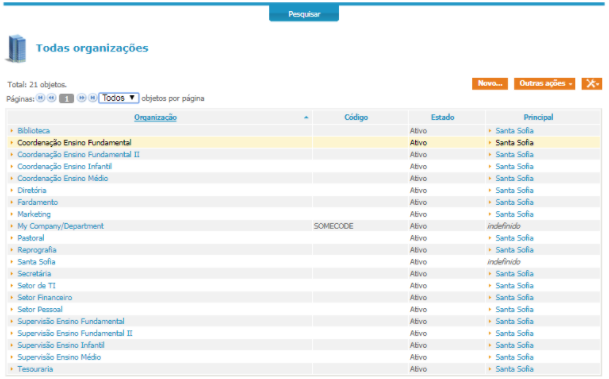
\includegraphics[scale=0.9]{Figuras/itop.png}
\label{organizacao}
\end{figure}

A imagem acima mostra como ficou as organizações inseridas no Itop. O campo principal informa qual a organização principal que no caso do projeto é a organização Santa Sofia, as outras organizações são organizações secundárias.

\subsection{Criação das localizações}
Com a criação das localizações é possível inserir os itens de configuração por localização geográfica, isso ajuda bastante na localização dos itens que estão em cada  setor da empresa. A imagem \ref{localidades} mostra as localidades da empresa.
\newpage

\begin{figure}[!h]
\centering
\caption[Localidades da empresa]{Localidades da Empresa}
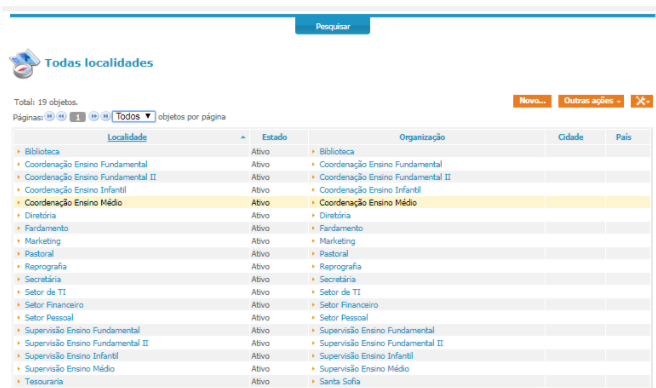
\includegraphics[scale=0.9]{Figuras/itop1.png}
\label{localidades}
\end{figure}
A imagem acima mostra todas as localizações da empresa que possui algum item de configuração.



\subsection{Criação das pessoas(usuários do sistema)}
Nessa etapa são inseridos os dados dos usuários no sistema. Essa etapa é importante para que se possa criar os perfis de acesso e as equipes, que ficarão responsáveis por executar determinados serviços. As imagens \ref{pessoas} e \ref{pessoas1} mostram como esse processo acontece.
\newpage

\begin{figure}[!h]
\centering
\caption[Criação de equipes ou pessoas]{Criação de equipes ou pessoas}
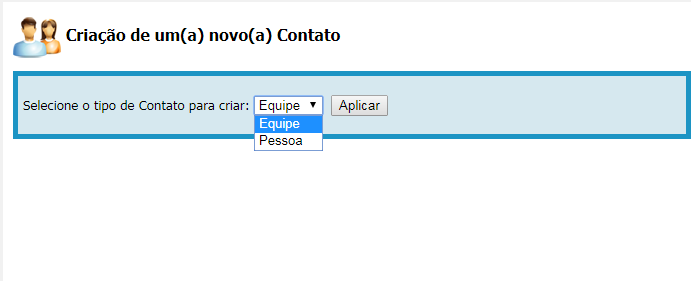
\includegraphics[scale=0.9]{Figuras/criacaodepessoas.png}
\label{pessoas}
\end{figure}


\newpage

\begin{figure}[!h]
\centering
\caption[Criação de usuários do sistema]{Criação de usuários do sistema}
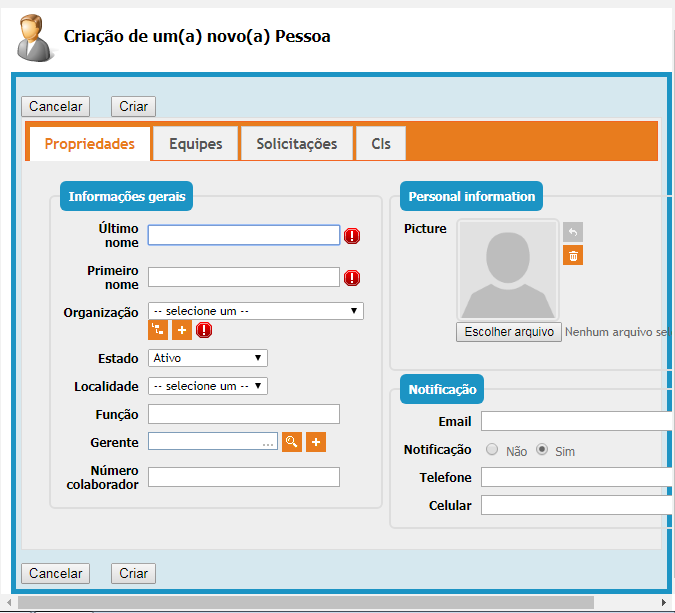
\includegraphics[scale=0.9]{Figuras/criacaodepessoas1.png}
\label{pessoas1}
\end{figure}

Como é possível observar a imagem \ref{pessoas} detalha o processo inicial de criação dos usuários do sistema. Já a imagem \ref{pessoas1} corresponde a tela seguinte, na qual os dados são inseridos.


\subsection{Criação dos itens de configuração}
Antes da realização do cadastro dos itens de configuração é necessário a criação dos objetos na seguinte ordem: fabricante, modelo e tipo dispositivo rede. Após essa etapa foram inserido os itens de configuração no sistema.
Finalizado os itens de configuração, iníciou a implantação da central de serviços.  Abaixo será apresentado um passa a passo da configuração da central de serviços.

\subsection{Criação do catálogo de serviços}

Com criação do catálogo de serviços torna-se possível apresentar uma relação dos serviços que o setor de TI pode prover aos demais funcionários da instituição, como também auxílio ao gestor de TI.

Como a empresa nunca teve um catálogo de serviços e os funcionários não estavam habituados, o catálogo desenvolvido foi bastante simples. 

No ITOP o catálogo de serviços consiste em uma lista, que uma determinada organização prestadora oferece aos seus clientes. Esses serviços são organizados em três níveis hierárquicos: primeiro nível, criação da familia de serviços  nomeada como: serviços de TI. Segundo nível, descrição  dos serviços ofertados e organização prestadora de serviços, que nesse caso foi o setor de TI. Terceiro nível, subserviços que são associados aos serviços ofertados. Nessa etapa é possível descrever se esse serviço é gerado através de um incidente ou de uma solicitação. Na imagem \ref{catalogo} é possíver ver o catálogo de serviços inícial.

\newpage

\begin{figure}[!h]
\centering
\caption[Catálogo de serviços]{Catálogo de Serviços}
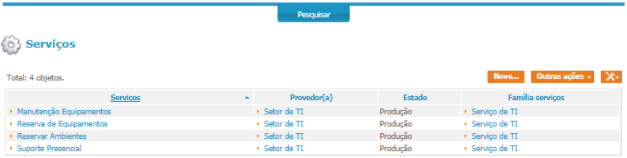
\includegraphics[scale=0.9]{Figuras/itop2.png}
\label{catalogo}
\end{figure}

A imagem acima mostra o catálogo de serviços, a organização provedora e a família de serviços pertencente.

\subsection{Definição de objetivos de níveis de serviços  e acordo de níveis de serviços}

Os objetivos de níveis de serviços são os prazos máximos para execução de uma ação sobre um ticket.  A definição de objetivos de níveis de serviços no ITOP utiliza duas métricas, time to own (TTO), que é o tempo entre a abertura do ticket e a sua associação ao um técnico e time to resolve (TTR), que  é o tempo entre a abertura do ticket e a sua solução . A imagem \ref{definicao} abaixo defini os objetivos de níveis de serviços.

\newpage

\begin{figure}[!h]
\centering
\caption[Definição de objetivos de níveis de serviços]{Definição de objetivos de níveis de serviços}
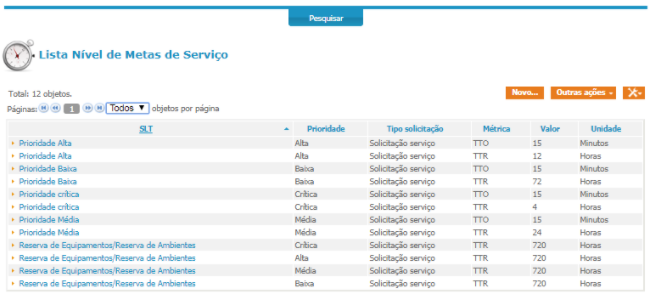
\includegraphics[scale=0.9]{Figuras/itop3.png}
\label{definicao}
\end{figure}

Assim sendo, para associação de um serviço há um técnico responsável por efetuá-lo. Foi definido um prazo máximo de 15 minutos após a abertura do ticket. Já para resolução dos serviços foram definidos os prazos corforme cada serviço ofertado e sua prioridade, por exemplo: para o serviço reserva de equipamentos foi delimitado um prazo de 30 dias para fechamento e resoluçao do ticket. Os colaboradores podem fazer uma reserva no maxímo de trinta dias de antecedência,motivo para esse prazo  ser elevado.  Os SLTS foram definidos em horas ou minutos, associados ao tipo de ticket e definido sua prioridade. 

O acordo de nível de serviço consistem em um agrupamento de SLTS, normalmente são utilizados para fazer uma distinção entre pacotes oferecidos aos clientes. Na imagem \ref{acordo} é exibido os acordos de níveis de serviços criados.

\newpage

\begin{figure}[!h]
\centering
\caption[Acordo de níveis de serviços]{Acordo de níveis de serviços}
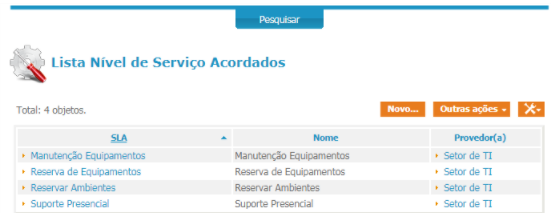
\includegraphics[scale=0.9]{Figuras/itop4.png}
\label{acordo}
\end{figure}
A imagem acima mostra a lista de acordos de níveis de serviços criados, o nome dos pacotes e a organização provedoras dos serviços. 

\subsection{Criação dos contratos com os clientes }

Os contratos com os clientes uniu as organizações clientes com as organizações provedora de serviços. Em suma, associou-se a lista de serviços prestados com os seus respectivos acordos de serviços. Na imagem \ref{criacao} é possível ver como ficou a criação do contrato com os clientes no ITOP .

\newpage

\begin{figure}[!h]
\centering
\caption[Contrato com os clientes]{Contrato com os clientes}
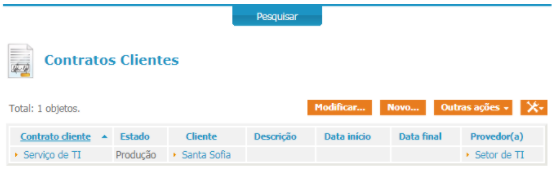
\includegraphics[scale=0.9]{Figuras/itop5.png}
\label{criacao}
\end{figure}

A imagem acima mostra a organização cliente e a organização provedora de serviços.

\subsection{Definição do modelo de entrega}

Na definição do modelo de entrega foi informado qual equipe irá atender os  clientes, porém só foi associado a um cliente um único modelo de entrega. A definição do modelo de entrega serviu para agrupar a equipe prestadora dos serviços com os clientes. Na imagem \ref{entrega} é pode-se observar a criação do modelo de entrega no ITOP .

\newpage

\begin{figure}[!h]
\centering
\caption[Modelo de Entrega]{Modelo de Entrega}
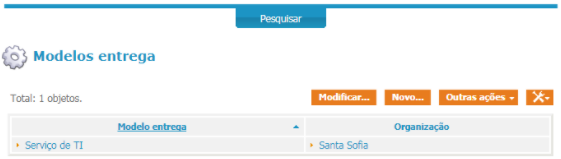
\includegraphics[scale=0.9]{Figuras/itop6.png}
\label{entrega}
\end{figure}

A imagem acima mostra o modelo de entrega produzido na instituição. No modelo foi definido as organizações atendidas pela equipe de TI e os clientes.

\subsection{Criação dos perfis de acessos}

No ITOP é possível que cada usuário faça a sua solicitação através de qualquer aparelho que esteja na rede de internet do colégio. Para isso, cada usuário do sistema tem que possuir um perfil de acesso.  De início foi criado uma conta para cada um dos funcionários da instituição, por meio dessas contas pode-se vincular um perfil de acesso. Na imagem \ref{perfil} é possível  ver os perfis de acessos oferecidos pelo ITOP. 

\newpage

\begin{figure}[!h]
\centering
\caption[perfil]{Perfis de Acessos}
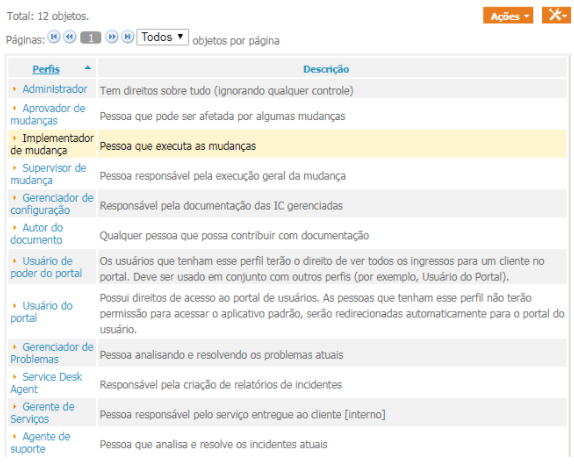
\includegraphics[scale=0.9]{Figuras/itop7.png}
\label{perfil}
\end{figure}

A imagem acima mostra todos os perfis de acesso que o ITOP permite e uma breve descrição de cada um. Com a criação dos perfis dos usuários o sistema  está pronto para uso.

\subsection{Detalhamentos das atividades executadas}

Para  entendimento de como foi executado o plano de atividades, dentro da instituição, foram produzidas duas tabelas que especificam cada atividade trabalhada durante o estágio, a carga horária, período de início e a conclusão das tarefas. Na tabela \ref{tab:atividades1} está descrita as atividades executada antes do uso do software ITOP.  Já na tabela \ref{tab:atividades2} está descrita as atividades trabalhadas com o software ITOP.
\index{tabelas!com quebra de pagina@com quebra de página}%
\index{tabelas!longas}%
\index{tabelas!package longtable@\eng{package} \pack{longtable}}%

\begin{longtable}[c]{p{4.7cm}cp{2.5cm}}
  %%%
  %%% firsthead -- essa seção aparece apenas no primeiro cabeçalho.
  %%%
  \caption{Atividades desenvolvidas\label{tab:atividades1}} \\
  \hline
  Atividades & Horas Execultadas & Período \\
  \hline\hline
  \endfirsthead
  %%%
  %%% head -- essa seção aparece nos demais cabeçalhos.
  %%%
  \caption[]{Atividades desenvolvidas (continuação)} \\
  \hline
  Atividades & Horas Execultadas & Período \\
  \hline\hline
  \endhead
  %%%
  %%% lastfoot -- essa seção aparece apenas no último rodapé.
  %%%
  \hline\hline
  \endlastfoot
  %%%
  %%% foot -- essa seção aparece nos demais rodapés.
  %%%
  \hline
  \multicolumn{3}{r}{\footnotesize{}continua na próxima página} \\
  \endfoot
\hline
Levantamento e estudo de material de apoio
(bibliográfico) necessário para implantação da ITIL. & 36 & Inicio: 01/11/2017 Fim: 09/11/2017\\
\hline
Levantamento dos recursos disponíveis. & 6 & Inicio: 10/11/2017
Fim: 10/11/2017\\
\hline
Montagem e formatação dos computadores que serão usados como servidor e servidor reserva. & 12 & Inicio: 13/11/2017
Fim: 14/11/2017\\
\hline
Processo de instalação dos software responsáveis pela montagem do gerenciamento de configuração e da central de serviços. & 12 & Inicio: 16/11/2017
Fim: 17/11/2017\\
\hline
Recolhimentos dos números de série de todos os ativos de TI, em todos os setores da empresa & 24 & Inicio: 18/11/2017
Fim: 23/11/2017\\
\hline
Criação de etiquetas e inserção nos ativos.  & 30 & Inicio: 24/11/2017
Fim: 29/11/2017\\
\hline
  
 \end{longtable}







\index{tabelas!com quebra de pagina@com quebra de página}%
\index{tabelas!longas}%
\index{tabelas!package longtable@\eng{package} \pack{longtable}}%

\begin{longtable}[c]{p{4.7cm}cp{2.5cm}}
  %%%
  %%% firsthead -- essa seção aparece apenas no primeiro cabeçalho.
  %%%
  \caption{Atividades desenvolvidas com o ITOP\label{tab:atividades2}} \\
  \hline
  Atividades & Horas Execultadas & Período \\
  \hline\hline
  \endfirsthead
  %%%
  %%% head -- essa seção aparece nos demais cabeçalhos.
  %%%
  \caption[]{Atividades desenvolvidas com o ITOP (continuação)} \\
  \hline
  Atividades & Horas Execultadas & Período \\
  \hline\hline
  \endhead
  %%%
  %%% lastfoot -- essa seção aparece apenas no último rodapé.
  %%%
  \hline\hline
  \endlastfoot
  %%%
  %%% foot -- essa seção aparece nos demais rodapés.
  %%%
  \hline
  \multicolumn{3}{r}{\footnotesize{}continua na próxima página} \\
  \endfoot
\hline
Estudo do funcionamento do ITOP & 12 & Inicio: 30/11/2017
Fim: 01/12/2017\\
\hline
Criação das organizações da empresa(Setores da empresa), utilizando o software ITOP. & 6 &Inicio: 04/12/2017
Fim: 04/12/2017\\
\hline
Criação das localizações dos itens de configuração na empresa(Setores onde se encontram os ICs). & 6 & Inicio: 05/12/2017
Fim : 05/12/2017\\
\hline
Inserção dos dados dos usuários do sistema  & 12 & Inicio: 06/12/2017
Fim: 07/12/2017\\
\hline
Criação dos tipos de itens de configuração no sistema e cadastros dos mesmos. & 30 & Inicio: 08/12/2017
Fim: 14/12/2017\\
\hline
Criação do catálogo de serviços  e elaboração dos SLTS e das SLA’s, para a central de serviços. & 12 & Inicio: 15/12/2017 Fim: 18/12/2017\\
\hline
Definição do modelo de entrega & 6 & Inicio : 19/12/2017
Fim : 19/12/2017\\
\hline
Treinamento da equipe de TI & 6 & Inicio : 20/12/2017
Fim : 20/12/2017\\
\hline
Criar as contas de usuários do Service Desk & 12 & Inicio : 21/12/2017
Fim: 22/12/2017\\
\hline
Disponibilizar o acesso aos usuários e criação dos perfis de cada colaborador no  Service Desk  & 12 &  Inicio: 08/01/2018
Fim: 09/01/2018\\
\hline
Treinamento para os colaboradores & 18 & Inicio: 10/01/2018
Fim: 12/01/2018\\
\hline
Criação de tutorial de uso do sistema, tanto para a equipe de TI, quanto para o restante dos funcionários  & 18 & Inicio: 15/ 01/2018
Fim: 17/01/2018\\
\hline
Montagem do relatório final e apresentação do mesmo ao supervisor do estágio. & 36 & Inicio: 01/11/2017
Fim: 25/01/2018\\
\hline
  
 \end{longtable}


Nas tabelas acima são apresentadas as sequências de passos para execução do plano de atividades desenvolvido na empresa.

\chapter{Conclusões}

\label{chap:conclusao}

Finalizado o período de estágio e concluido todas as atividades propostas, foi possível perceber o quanto os conhecimentos adquiridos durante os anos de graduação são importantes para a formação de um  profissional.  O estágio proporcionou conhecimentos relevantes para a vida profissional do estagiário, uma vez que propriciou o enfrentamento dos desafios do mercado de trabalho, fazendo com que se construisse autonomia para lidar com os problemas que possam surgir na execução de projetos.

A metodologia de trabalho caracterizou-se pela definição de etapas, que foram superadas uma a uma  seguindo o planejamento inicial do estágio. A implantação do ITOP ocorreu de maneira esperada, tendo em vista que proporcionou ao colégio  um controle maior dos seus ativos de TI, facilitando o trabalho do setor de tecnologia. A empresa passou a possuir uma central de serviços que atende as necessidades da organização.  A metodologia ITIL facilitou o processo de implantação, além de colocar a empresa em um patamar mais elevado tecnologicamente. Assim, os resultados obtidos com a implementação da ITIL foram significativos, pois houve a satisfação de todos que fizeram parte desse projeto. 




%\appendix
%\chapter{Apêndice}\label{ane:relatorio}



\bibliographystyle{estilo_ABNT}
\bibliography{refs}
\addcontentsline{toc}{chapter}{Bibliografia}

\end{document}

